%% @Author: Ines Abdeljaoued Tej
%  @Date:   2018-02
%% @Class:  PFE de l'ESSAI - Universite de Carthage, Tunisie.

\documentclass[a4paper, oneside, frenchb]{report}

\providecommand{\keywords}[1]{\textbf{\textit{Mots cl\'es---}} #1}

\usepackage[nottoc]{tocbibind}

\usepackage[frenchb]{babel}
\textwidth 17cm
\textheight 24cm
\topmargin -1cm
\oddsidemargin -0.5cm
%\DefineBibliographyStrings{french}{in={dans},inseries={dans}}

% set font encoding for PDFLaTeX or XeLaTeX
\usepackage{ifxetex}
\ifxetex
  \usepackage{fontspec}
\else
  \usepackage[T1]{fontenc}
  \usepackage[utf8]{inputenc}
  \usepackage{lmodern}
\fi


\newcommand{\reportTitle} {%
  %\textsc{Graduation Project}
  \textsc{Projet de Fin d'\'etudes}
}

\newcommand{\reportAuthor} {%
  FirstName \textsc{LastName}%
}

\newcommand{\reportSubject} {%
  Le titre du rapport \\ Titre%
}

\newcommand{\dateSoutenance} {%
  12/06/2018%
}

\newcommand{\studyDepartment} {%
  Entreprise d'accueil %Statistique
}

\newcommand{\ESSAI} {%
  %Higher School of Statistics and Information Analysis
  Ecole Sup\'erieure de la Statistique et de l'Analyse de l'Information
}

%\newcommand{\codePFE} {% Reference
%  Code PFE%
%}

\newcommand{\juryPresident} {%
  M. Ben Foulen \textsc{Foulenia}%
}
\newcommand{\juryPresidentDesc} {%
  Pr\'esident%
}

\newcommand{\juryMemberOne} {%
  Mme Ben Foulena \textsc{Foulen}%
}
\newcommand{\juryMemberOneDesc} {%
  Encadrant %Mentor
}

\newcommand{\juryMemberTwo} {%
  M. Ben Foulen \textsc{Fouleni}%
}
\newcommand{\juryMemberTwoDesc} {%
  Rapporteur% Examiner, Reporter
}

\newcommand{\specialcell}[1]{%
  \begin{tabularx}{\textwidth}{@{}X@{}}#1\end{tabularx}%
}

%%%%%%%%%%%%%%%%%%%%%%%%%%%%%%%%%%%%%%%%%%%%%%%%%%%%%%%
% Add your own commands here
%%%%%%%%%%%%%%%%%%%%%%%%%%%%%%%%%%%%%%%%%%%%%%%%%%%%%%%
\newcommand{\MyCommand} {%
  Does nothing really%
}


% used in maketitle
\title{\reportSubject}
\author{\reportAuthor}

% Enable SageTeX to run SageMath code right inside this LaTeX file.
% documentation: http://mirrors.ctan.org/macros/latex/contrib/sagetex/sagetexpackage.pdf
%\usepackage{sagetex}
\usepackage{graphics}
\usepackage{graphicx}

\begin{document}

\thispagestyle{empty}
\begin{titlepage}
\begin{center}


%%%%%%%%%%%%%%%%%%%%%%%%%%%%%%%%%%%%%%%%%%%%%%%
% THE HEADER
%%%%%%%%%%%%%%%%%%%%%%%%%%%%%%%%%%%%%%%%%%%%%%%


\includegraphics[width=2cm, height=1.5cm]{embleme.jpg}\\
\vspace{0.5cm}

{%
  \fontsize{9pt}{9pt}\selectfont%
  \begin{tabular}{c}
    R\'epublique Tunisienne \\
    Minist\`ere de l'Enseignement Supérieur et de la Recherche Scientifique \\%
    Universit\'e de Carthage - \ESSAI{}  \\
  \end{tabular}
}

\vspace{1cm}


\includegraphics[width=4cm, height=2.5cm]{universite-carthage.jpg}


%%%%%%%%%%%%%%%%%%%%%%%%%%%%%%%%%%%%%%%%%%%%%%%
% THE PAGE CONTENT
%%%%%%%%%%%%%%%%%%%%%%%%%%%%%%%%%%%%%%%%%%%%%%%

\vspace{30pt} {%
  \renewcommand*{\familydefault}{\defaultFont}
  \fontsize{46pt}{46pt}\selectfont%
  % MEMOIRE\\%
  %\reportTitle{}%\\\textsc{Report}\\%
}

\vspace{10pt}
\textbf{\textit{Rapport de Projet de Fin d'Etudes soumis afin d'obtenir le titre d'}}\\

\vspace{10pt}
Ing\'enieur en Statistique et Analyse de l'Information\\


\includegraphics[width=2.5cm, height=2.5cm]{logo-essai.jpg}\\

\vspace{30pt}
\textbf{\textit{par}}\\
\vspace{10pt} {%
  \fontsize{18pt}{18pt}\selectfont%
  \textbf{\reportAuthor}\\
}%

\vspace{10pt} {%
  \renewcommand*{\familydefault}{\defaultFont}
  \fontsize{27pt}{27pt}\selectfont%
  \rule{0.5\textwidth}{.4pt}\\
  \vspace{10pt}
  \reportSubject{}\\%
  \vspace{10pt}
  \rule{0.5\textwidth}{.4pt}
}

\vspace{10pt}
Soutenu le~\dateSoutenance~devant le Jury compos\'e de :\\
%Soutenu le \dateSoutenance, devant la commission d'examen:\\
\vspace{20pt}
\begin{tabular}{p{0.3\linewidth} p{0.15\linewidth}}
  \juryPresident{} & \juryPresidentDesc{}\\
  \juryMemberOne{} & \juryMemberOneDesc{}\\
  \juryMemberTwo{} & \juryMemberTwoDesc{}\\
\end{tabular}

\vfill

\vspace{30pt}%
\textbf{\textit{Projet de Fin d'Etudes fait \`a}}\\

\vspace{10pt}
(\studyDepartment)\\

\end{center}
\end{titlepage}

% ###############################
% # HELP COMMANDS               #
% ###############################
%
% -1 \part{part}
%  0 \chapter{chapter}
%  1 \section{section}
%  2 \subsection{subsection}
%  3 \subsubsection{subsubsection}
%  4 \paragraph{paragraph}
%  5 \subparagraph{subparagraph}


%%%%%%%%%%%%%%%%%%%%%%%%%%%%%%%%%%%%%%%%%%%%%%%%%%%%%%%
% Dédicace et Remerciements
%%%%%%%%%%%%%%%%%%%%%%%%%%%%%%%%%%%%%%%%%%%%%%%%%%%%%%%

%\chapter*{Dedication}
\chapter*{D\'edicace}
%\addcontentsline{toc}{chapter}{Dedication}
\thispagestyle{empty}
%
%For all they have endured to satisfy all my needs and wishes

\begin{center}
  Put your dedication lines here ~\\
  And try to be expressive ;) ~\\


  Lorem ipsum dolor sit amet, consectetur adipisicing elit, sed do eiusmod ~\\
  tempor incididunt ut labore et dolore magna aliqua. Ut enim ad minim veniam, ~\\
  quis nostrud exercitation ullamco laboris nisi ut aliquip ex ea commodo ~\\
  consequat. Duis aute irure dolor in reprehenderit in voluptate velit esse ~\\
  cillum dolore eu fugiat nulla pariatur. Excepteur sint occaecat cupidatat non ~\\
  proident, sunt in culpa qui officia deserunt mollit anim id est laborum ~\\
\end{center}
%
%\nopagebreak{%
% And maybe a quote here
% \raggedright\hspace{5.75cm} To all of you,~\\

%\chapter*{Thanks}
\chapter*{Remerciements}
%\addcontentsline{toc}{chapter}{Thanks}
\thispagestyle{empty}
%
And put your thanks here. ~\\

Lorem ipsum dolor sit amet, consectetur adipisicing elit, sed do eiusmod
tempor incididunt ut labore et dolore magna aliqua. Ut enim ad minim veniam,
quis nostrud exercitation ullamco laboris nisi ut aliquip ex ea commodo
consequat. Duis aute irure dolor in reprehenderit in voluptate velit esse
cillum dolore eu fugiat nulla pariatur. Excepteur sint occaecat cupidatat non
proident, sunt in culpa qui officia deserunt mollit anim id est laborum. Lorem ipsum dolor sit amet, consectetur adipisicing elit, sed do eiusmod
tempor incididunt ut labore et dolore magna aliqua. Ut enim ad minim veniam,
quis nostrud exercitation ullamco laboris nisi ut aliquip ex ea commodo
consequat. Duis aute irure dolor in reprehenderit in voluptate velit esse
cillum dolore eu fugiat nulla pariatur. Excepteur sint occaecat cupidatat non
proident, sunt in culpa qui officia deserunt mollit anim id est laborum.



%%%%%%%%%%%%%%%%%%%%%%%%%%%%%%%%%%%%%%%%%%%%%%%%%%%%%%%
% Divers chapitres
%%%%%%%%%%%%%%%%%%%%%%%%%%%%%%%%%%%%%%%%%%%%%%%%%%%%%%%

\tableofcontents

\chapter{Introduction}
\label{chap:general_intorduction}
\markboth{\MakeUppercase{Introduction}}{}%
\addcontentsline{toc}{chapter}{Introduction}%

%Welcome to \Ac{ESSAI}. ~\\
%Again, welcome to \Ac{ESSAI}. ~\\
%Your introduction goes here. ~\\

Lorem ipsum dolor sit amet, consectetur adipisicing elit, sed do eiusmod
tempor incididunt ut labore \cite{jenkins2004} et dolore magna aliqua. Ut enim ad minim veniam, du chapitre \ref{chap:general_intorduction}
quis nostrud exercitation ullamco laboris nisi ut aliquip ex ea commodo
consequat \cite{hui}. Duis aute irure dolor in reprehenderit in voluptate v.


Voici une référence à l'image de la figure \ref{fig:pictureTwo} page \pageref{fig:pictureTwo} et une autre vers la partie \ref{chapter2} page \pageref{chapter2}.
On peut citer un livre\, \cite{caillois1} et on précise les détails à la fin du rapport dans la partie références.
Voici une note\,\footnote{Texte de bas de page} de bas de page\footnote{J'ai bien dit bas de page}.


\begin{itemize}
  \item The individual entries are indicated with a black dot, a so-called bullet.
  \item The text in the entries may be of any length.
\end{itemize}

\chapter{Chapitre Un}%
\label{chap:chapterone}

%%%%%%%%%%%%%%%%%%%%%%%%%%%%
% SECTION                  %
%%%%%%%%%%%%%%%%%%%%%%%%%%%%
\section{Section une}
\label{chap:sectionone}

\subsection{Sub section One}

And your chapter one goes here \cite{web001,Nom2012}. \\
  Lorem ipsum dolor sit amet, consectetur adipisicing elit, sed do eiusmod
  tempor incididunt ut labore et dolore magna aliqua. Ut enim ad minim veniam, quis nostrud exercitation ullamco laboris nisi ut aliquip ex ea commodo consequat. Duis aute irure dolor in reprehenderit in voluptate velit esse
  cillum dolore eu fugiat nulla pariatur. Excepteur sint occaecat cupidatat non
  proident, sunt in culpa qui officia deserunt mollit anim id est laborum.

  \begin{figure}[h]%
    \center%
    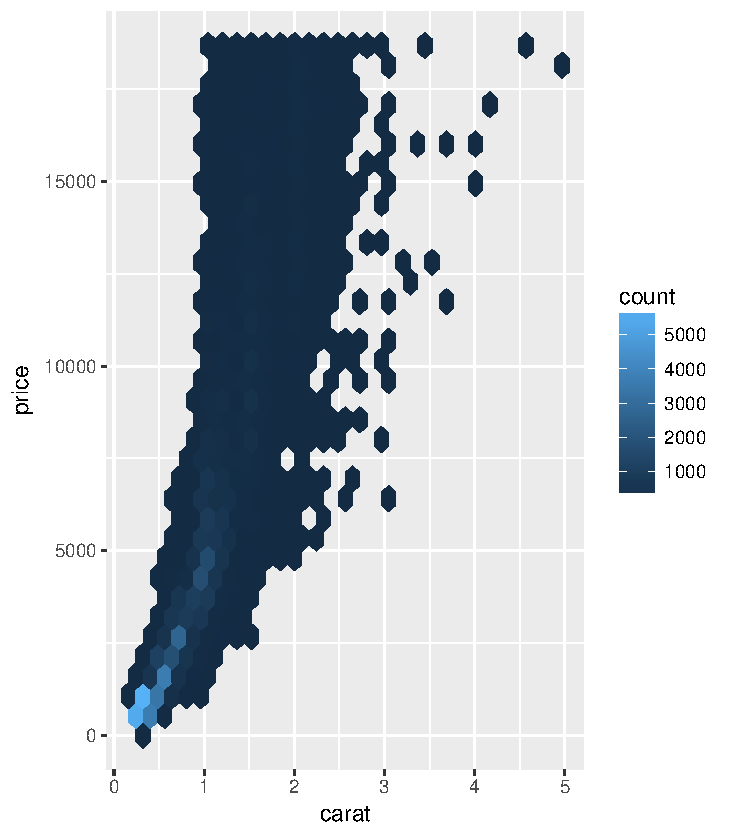
\includegraphics[width=0.3\textwidth]{diamonds.pdf}
    \caption[This is a test image]{Test Image}\label{fig:test}%
  \end{figure}


\begin{table}
\begin{tabular}{cc}
A & B \\
C & D
\end{tabular}
\caption{Test Table}
\end{table}

 \subsection{Sub section Two}

  This is a second subsection\cite{gen1972}, \cite{schaeffer99}. ~\\
  Lorem ipsum dolor sit amet, consectetur adipisicing elit, sed do eiusmod
  tempor incididunt ut labore et dolore magna aliqua. Ut enim ad minim veniam,
  quis nostrud exercitation ullamco laboris nisi ut aliquip ex ea commodo
  consequat. Duis aute irure dolor in reprehenderit in voluptate velit esse
  cillum dolore eu fugiat nulla pariatur. Excepteur sint occaecat cupidatat non
  proident, sunt in culpa qui officia deserunt mollit anim id est laborum.

  \begin{description}\addtolength{\itemsep}{-0.35\baselineskip}%
    \item[\textbullet~\bfseries Menu Item] \hfill \\%
      Menu Description.~\\%
      {\textbf{Focus topics:~}\emph{Topic one, topic two, topic three, ...}}%
    %
    \item[\textbullet~\bfseries Menu Item] \hfill \\%
      Menu Description.~\\%
      {\textbf{Focus topics:~}\emph{Topic one, topic two, topic three, ...}}%
    %
    \item[\textbullet~\bfseries Menu Item] \hfill \\%
      Menu Description.~\\%
      {\textbf{Focus topics:~}\emph{Topic one, topic two, topic three, ...}}%
  \end{description}

  Also bullets such as:%
  \begin{itemize}\addtolength{\itemsep}{-0.35\baselineskip}%
    \item One%
    \item Two%
    \item Three%
    \item Four%
    \item \ldots%
  \end{itemize}%
  %
\subsection{powers series} \label{subsection}

\begin{equation} \label{eq:1}
\sum_{i=0}^{\infty} a_i x^i
\end{equation}

The equation \ref{eq:1} is a typical power series.

\chapter*{Autre chapitre}
\label{chapter2}
\markboth{\MakeUppercase{Autrechap}}{}%
\addcontentsline{toc}{chapter}{Autre Chapitre}%

\chapter*{Conclusion}
\label{chap:conclusion}
\markboth{\MakeUppercase{Conclusion}}{}%
\addcontentsline{toc}{chapter}{Conclusion}
  And a very interesting conclusion here\@. ~\\
  Lorem ipsum dolor sit amet, consectetur adipisicing elit, sed do eiusmod
  tempor incididunt ut labore et dolore magna aliqua. Ut enim ad minim veniam,
  quis nostrud exercitation ullamco laboris nisi ut aliquip ex ea commodo
  consequat.

\chapter*{Annexe}
\label{chap:appendix}
\markboth{\MakeUppercase{Annexe}}{}
\addcontentsline{toc}{chapter}{Annexe}

  An appedix if you need it. ~\\

  Lorem ipsum dolor sit amet, consectetur adipisicing elit, sed do eiusmod
  tempor incididunt ut labore et dolore magna aliqua. Ut enim ad minim veniam,
  quis nostrud exercitation ullamco laboris nisi ut aliquip ex ea commodo.


%%%%%%%%%%%%%%%%%%%%%%%%%%%%%%%%%%%%%%%%%%%%%%%%%%%%
% Don't touch this, it is auto generated
%%%%%%%%%%%%%%%%%%%%%%%%%%%%%%%%%%%%%%%%%%%%%%%%%%%%
\nocite{*}

%\phantomsection{}
%\addcontentsline{toc}{chapter}{Webography}
%\printbibliography[title={Webography},type=online]

%\phantomsection{}
%\addcontentsline{toc}{chapter}{Bibliography}
%\printbibliography[title={Bibliography},nottype=online]

%\printbibheading %exemple de bibliographie divisée en sections. Pour ajouter des oeuvres non citées,utiliser \nocite

%\printbibliography[keyword=pratique,heading=subbibliography,title={Théories littéraires dans les jeux vidéo}]
%\printbibliography[keyword=litteraire,heading=subbibliography,title={Narratologie et structuralisme}]

%\printbibliography[keyword=jeu,heading=subbibliography,title={\emph{Games studies}}]

\bibliographystyle{apalike}
\bibliography{Biblio.bib}

\cleardoublepage%

\addtocontents{toc}{\protect\setcounter{tocdepth}{3}}

%\newpage

\begin{abstract}
Insérer un résumé en Français \\

\keywords{Ici mettre cinq mots clés}
\end{abstract}



\end{document}